\documentclass{template/han}

\title{
Casus RDI 2019 \newline
\large Video-on-demand internetplatform ODISEE
}
\def\docenten{
Marco Engelbart \newline
Mark Giessen \newline
Bram Laumans
}
\def\vak{
ADB-DT
}
\author{
Nick Hartjes (423064) \newline
Marc Groenhout (527698) \newline
Joey Stoffels (609589)
}
\date{\today}

\begin{document}
    \newpage
    \maketitle

    %=================o ~~
    \newpage
    \tableofcontents

    %=================o ~~
    \newpage
    \section{Opdracht 1: Bevragingen}
    \label{opdracht1}
    \paragraph{
        Maak voor iedere query die je schrijft minimaal ��n alternatieve implementatie indien mogelijk en vergelijk de queryplannen.
        Kies op basis van het queryplan, performance en onderhoudbaarheid van de code de juiste query en verklaar jouw keuze.
    }
    \subsection{Opdracht 01}

Geef van een film, de hele reeks waar die bij hoort met volgnummer en in de juiste volgorde.
Indien hij niet in een reeks zit, is de lijst gewoon ��n lang met volgnummer 1.
Dit moet ��n statement worden die van een variabel ID de reeks geeft zoals onderstaand voorbeeld:
DECLARE @MovieInReeks INT = 207989;


\begin{lstlisting}
-- jouw statement hier levert onderstaand resultaat:

ITEM_ID		TITLE				Volgnummer
207992		Matrix, The				1
207989		Matrix Reloaded, The			2
207991		Matrix Revolutions, The		3
\end{lstlisting}

\subsubsection{Versie 01}

TODO: Marc

\lstinputlisting[language=SQL]{sql/marc/opdracht-01-01.sql}
\begin{figure}
    \centering
    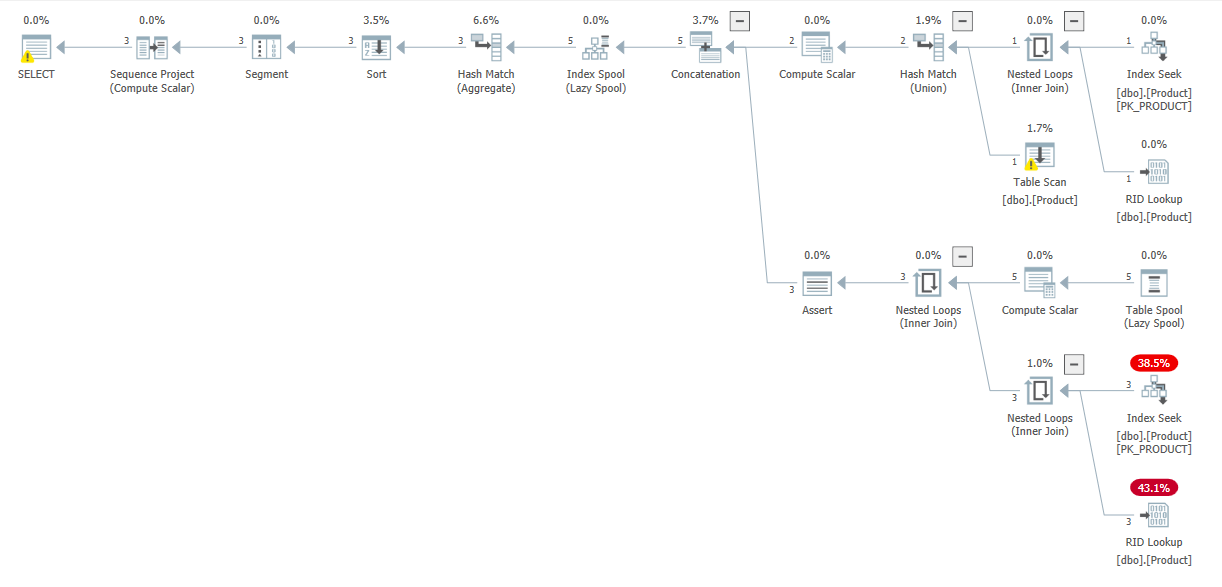
\includegraphics[width=1\textwidth]{image/marc/opdracht-01.PNG}
    \caption{Queryplan Opdracht 01 Versie 01}
\end{figure}

\subsubsection{Versie 02}
TODO: Joey

\lstinputlisting[language=SQL]{sql/joey/opdracht-01-01.sql}
\begin{figure}
    \centering
    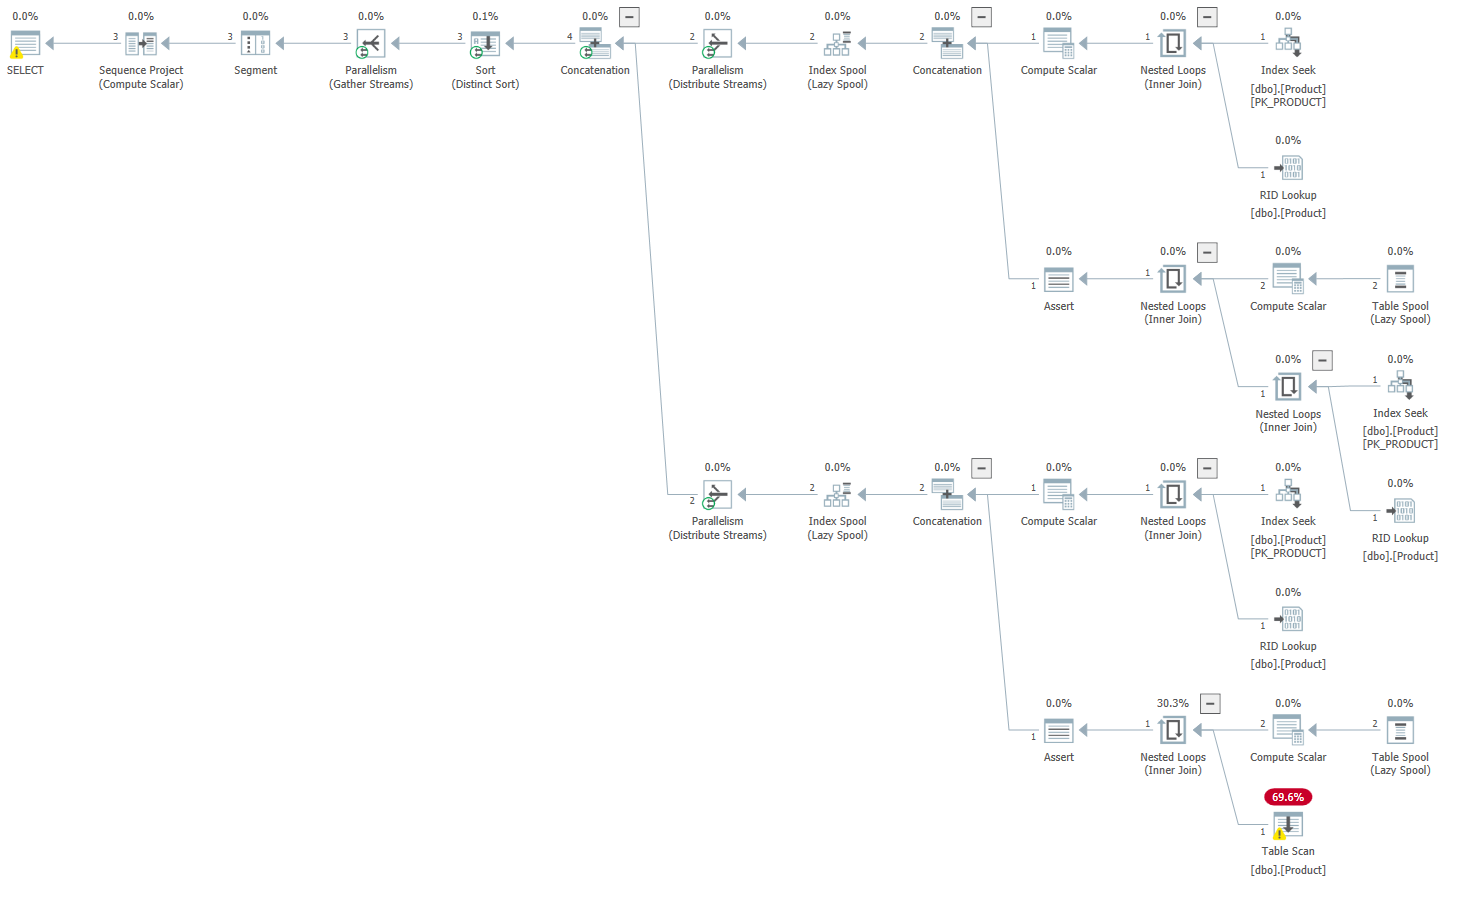
\includegraphics[width=1\textwidth]{image/joey/opdracht-01.PNG}
    \caption{Queryplan Opdracht 01 Versie 02}
\end{figure}


\subsubsection{Versie 03}

    De intentie van deze query was om geen CTE te gebruiken. In dit alternatief maken we gebruik van een tijdelijke tabel.
    Na het aanmaken van van de tijdelijke tabel worden er 2 while loops gedraaid. Bij de eerste loop word er gekeken of er een vorige film is.
    Als die er is, word die opgeslagen in de tijdelijke tabel, en herhaald hij de loop tot het punt komt dat er geen vorige film meer is.
    Hetzelfde doet hij met vervolg films, als deze er zijn word die ook in de tijdelijke tabel opgeslagen.
    Uiteindelijk word de tijdelijke tabel uitgevraagd, en krijg je de lijst met films te zien.
    Als laatste word de tijdelijke tabel verwijderd.

\lstinputlisting[language=SQL]{sql/nick/opdracht-01-01.sql}

\subsubsection{Conclusie}

\begin{tabular}{ || l | l | l | l | l | l | l | l | l | l | l | l | 1 | 1 | l | 1 | 1 || }
    \hline
    \textbf{Statement} & \textbf{Est Cost \%} & \textbf{Compile Time} & \textbf{Duration} &
    \textbf{CPU} & \textbf{Est CPU Cost \%} &
    \textbf{Est IO Cost \%} \\
    \hline
    \hline
    Versie01  & 0,0\%  & 12  & 40  & 40  & 4,9\% & 0,0\% \\
    \hline
    Versie02  & 100,0\%  & 20  & 76  & 75  & 95,1\% & 100,0\%  \\
    \hline
\end{tabular}
\newline
\newline
\begin{tabular}{ || l | l | l | l | l | l | l | l | l | l | l | l | 1 | 1 | l | 1 | 1 || }
    \hline
    \textbf{Statement} &  \textbf{Est Rows} & \textbf{Actual Rows} & \textbf{RID Lookups} &
    \textbf{Parallel} & \textbf{Sort} &
    \textbf{Table Scan} & \textbf{Hash Match} \\
    \hline
    \hline
    Versie01  & 77.765  & 3  & 2  & 0  & 1  & 1  & 2 \\
    \hline
    Versie02  & 1.157.780  & 3  & 3  & 5  & 1  & 1  & 0 \\
    \hline
\end{tabular}


HIer komt dus een lang verhaal over welke query het beste is, en waarom

    \clearpage
    \subsection{Opdracht 02}

\paragraph{
Geef het statement dat per land het maandgebruik over 12 maanden geeft met daarbij het percentage dat die maand uitmaakt van het totaal van die 12 maanden.
Hier zijn twee interpretaties mogelijk: per land de afgelopen 12 maanden in rijen, hier onder de uitdraai voor b.v. �Netherlands� uitgevoerd in april 2019.
}

\begin{lstlisting}
    Year	Month	ItemsPerMonth	PercentageOfTotal
    2018	4	60		4.44%
    2018	5	60		4.44%
    2018	6	60		4.44%
    2018	7	56		4.14%
    2018	8	132		9.76%
    2018	9	155		11.46%
    2018	10	141		10.43%
    2018	11	138		10.21%
    2018	12	148		10.95%
    2019	1	137		10.13%
    2019	2	117		8.65%
    2019	3	148		10.95%
\end{lstlisting}

\lstinputlisting[language=SQL]{sql/nick/opdracht-01-02a.sql}
\lstinputlisting[language=SQL]{sql/marc/opdracht-01-02a.sql}
\lstinputlisting[language=SQL]{sql/joey/opdracht-01-02a.sql}
    \clearpage
    \subsection{Opdracht 02b}
Een mooier alternatief is een statement dat per land de percentages en totalen geeft over een jaar in kolommen.

\begin{lstlisting}
    -- jouw statement hier levert b.v. onderstaand resultaat voor 2017

    Countryname  January	Feburary  March    April    May    June    July    August  September  October  November  December  TotalItems
    Chile         9.76%    8.22%   10.06%    9.07%   9.26%   8.38%   8.91%    7.75%    7.28%     7.09%     7.53%    6.68%     3638
    Greece        9.67%    7.69%    9.06%    8.49%   8.49%   7.92%   9.06%    8.49%    8.40%     7.78%     7.78%    7.17%     2120
    Poland        9.93%    7.94%    9.41%    8.82%   8.82%   8.24%   8.24%    7.72%    7.72%     7.72%     7.72%    7.72%     1360
    Netherlands   8.38%    7.26%    8.94%    8.38%   8.38%   7.82%   8.94%    8.38%    8.38%     8.38%     8.38%    8.38%      716
\end{lstlisting}

\subsubsection{Versie 01}
TODO: Nick
\lstinputlisting[language=SQL]{sql/nick/opdracht-01-02b-v1.sql}
\begin{figure}[H]
    \centering
    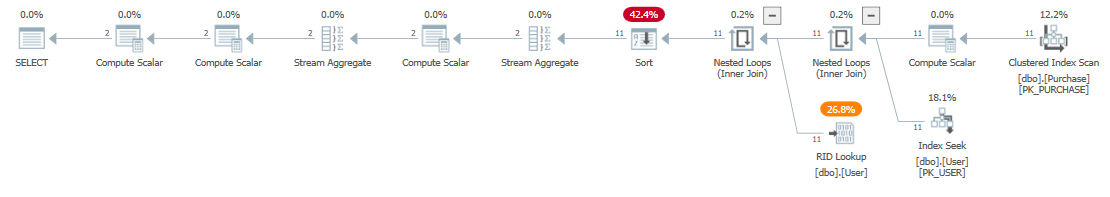
\includegraphics[width=1\textwidth]{image/nick/opdracht-02b.PNG}
    \caption{Queryplan Opdracht 02b Versie 01}
\end{figure}

\subsubsection{Versie 02}

    In onderstaande versie wordt er gebruik gemaakt van een PIVOT. Bij een PIVOT worden rijen omgezet naar kolommen. Indien er geen verkopen
    zijn in een bepaalde maand, dan wordt er een standaard waarde van 0.00\% getoond. Door in de FROM clausule de juiste set met gegevens
    aan te leveren, wordt in het SELECT statement enkel en alleen nog de gewenste informatie uit de juiste kolommen opgevraagd.

\lstinputlisting[language=SQL]{sql/marc/opdracht-01-02b.sql}
\begin{figure}[H]
    \centering
    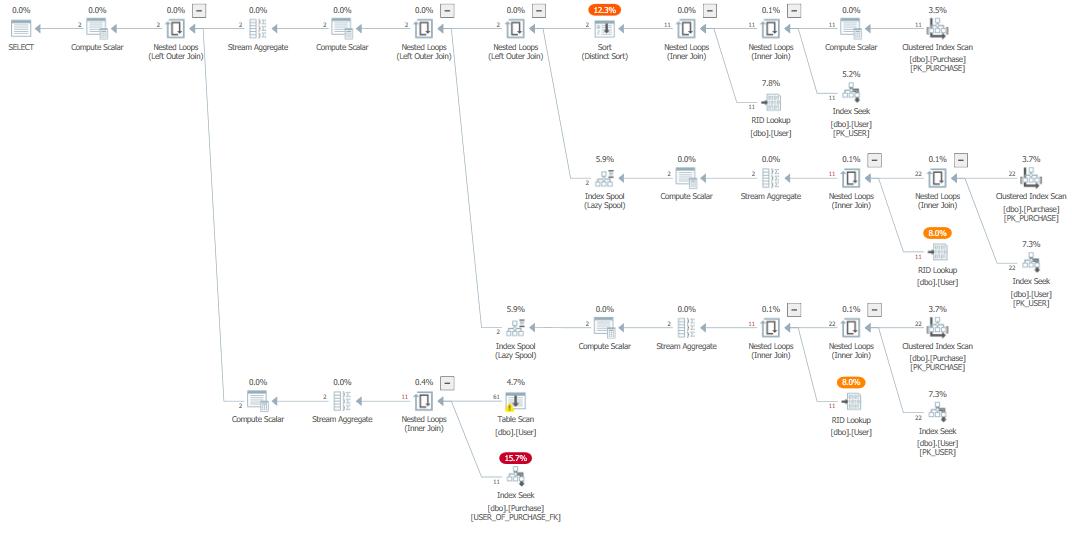
\includegraphics[width=1\textwidth]{image/marc/opdracht-02b.PNG}
    \caption{Queryplan Opdracht 02b Versie 02}
\end{figure}

\subsection{Conclusie}
Versie 01 presteert met 22\% van de totale duur van de gehele batch aanzienlijk sneller dan versie 02 welke 78\% van de duur nodig heeft.
Uit het queryplan wordt duidelijk dat versie 02 in het beginstadium net iets beter presteert. Deze voert een 'Index Seek (NonClustered)' uit
voor 2 van de 11 records in de User tabel. Hetzelfde geldt voor de 'RID Lookup (Heap)' welke eveneens voor 2 van de 11 records informatie
uit de User tabel ophaalt. Na deze stap doorloopt versie 01 echter een eenvoudig proces zonder extra 'Nested Loops' en de extra ballast
welke hieraan vooraf gaat zoals een 'Filter', 'Clustered Index Scan' en een 'Table Scan'. Derhalve kan worden gesteld dat versie 01
beter preseteert dan versie 02. De onderhoudbaarheid van versie 01 is eveneens beter dan die van versie 02, niet alleen omdat de structuur
helder en overzichtelijk is, maar ook vanwege het gebruik van een CTE waardoor een duidelijke resultset terug wordt gegeven.\\
\\
\begin{tabular}{ || l | l | l | l | l | l | l | l | l | l | l | l | 1 | 1 | l | 1 | 1 || }
    \hline
    \textbf{Statement} & \textbf{Est Cost \%} & \textbf{Compile Time} & \textbf{Duration} &
    \textbf{CPU} & \textbf{Est CPU Cost \%} &
    \textbf{Est IO Cost \%} \\
    \hline
    \hline
    Versie01  & 22,5\%  & 12  & 2  & 2  & 9,8\% & 28,9\% \\
    \hline
    Versie02  & 77,5\%  & 35  & 8  & 3  & 90,2\% & 71,1\%  \\
    \hline
\end{tabular}
\newline
\newline
\begin{tabular}{ || l | l | l | l | l | l | l | l | l | l | l | l | 1 | 1 | l | 1 | 1 || }
    \hline
    \textbf{Statement} &  \textbf{Est Rows} & \textbf{Actual Rows} & \textbf{RID Lookups} &
    \textbf{Parallel} & \textbf{Sort} &
    \textbf{Table Scan} & \textbf{Hash Match} \\
    \hline
    \hline
    Versie01  & 2  & 2  & 1  & 0  & 1  & 0  & 0 \\
    \hline
    Versie02  & 2  & 2  & 3  & 0  & 1  & 1  & 0 \\
    \hline
\end{tabular}
    \clearpage
    \subsection{Opdracht 03}

\paragraph{
Geef de 10 films met de hoogste mediaan van hun reviews. Wat zegt dit getal over een film?
}

\lstinputlisting[language=SQL]{sql/nick/opdracht-03.sql}
\lstinputlisting[language=SQL]{sql/marc/opdracht-03.sql}
\lstinputlisting[language=SQL]{sql/joey/opdracht-03.sql}
    \clearpage
    \subsection{Opdracht 04}

\paragraph{
In de oorspronkelijke data van IMDB staat in Imported_Director_Genre een veld Prob. Dit geeft de kans dat een film in deze database van dat genre is. Onderstaande query geeft de resultaten voor Sergio Leone.
\begin{lstlisting}
    SELECT *
    FROM myimdb.dbo.Imported_Director_Genre
    WHERE did = 46046
    ORDER BY Prob
\end{lstlisting}
Staan deze gegevens in de juiste volgorde? Maak een query die deze gegevens produceert vanuit jouw eigen database op volgorde van kans, met de grootste kans bovenaan.
}

\lstinputlisting[language=SQL]{sql/nick/opdracht-01-04.sql}
\lstinputlisting[language=SQL]{sql/marc/opdracht-01-04.sql}
\lstinputlisting[language=SQL]{sql/joey/opdracht-01-04.sql}
    \clearpage
    \subsection{Opdracht 05a}

Vermoedelijk zijn niet alle Film ID�s in gebruik. Geef het statement dat de langste aaneengesloten reeks geeft van Film ID�s in jouw database.

\subsubsection{Versie 01}

TODO: Marc

\lstinputlisting[language=SQL]{sql/marc/opdracht-01-05a.sql}
\begin{figure}
    \centering
    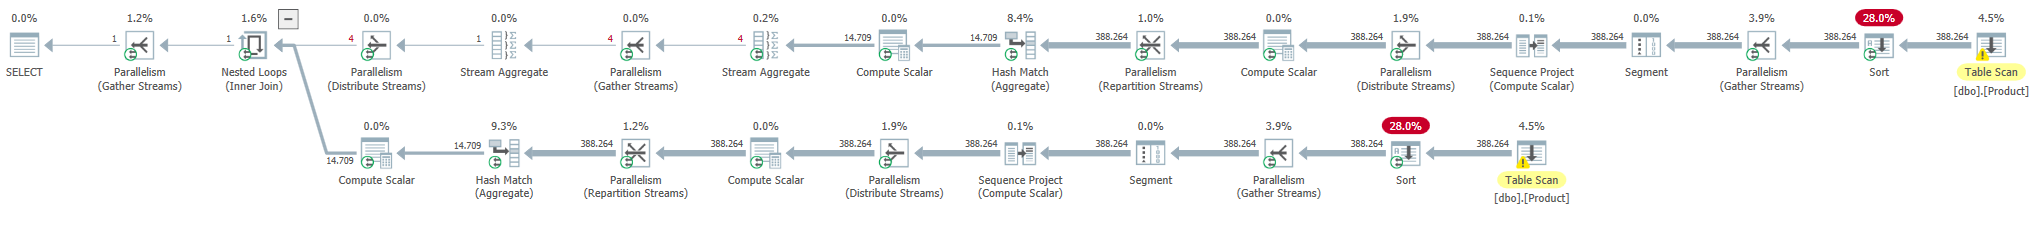
\includegraphics[width=1\textwidth]{image/marc/opdracht-05a.PNG}
    \caption{Queryplan Opdracht 05 Versie 01}
\end{figure}

\subsubsection{Versie 02}

TODO: Joey

\lstinputlisting[language=SQL]{sql/joey/opdracht-01-05a.sql}
\begin{figure}
    \centering
    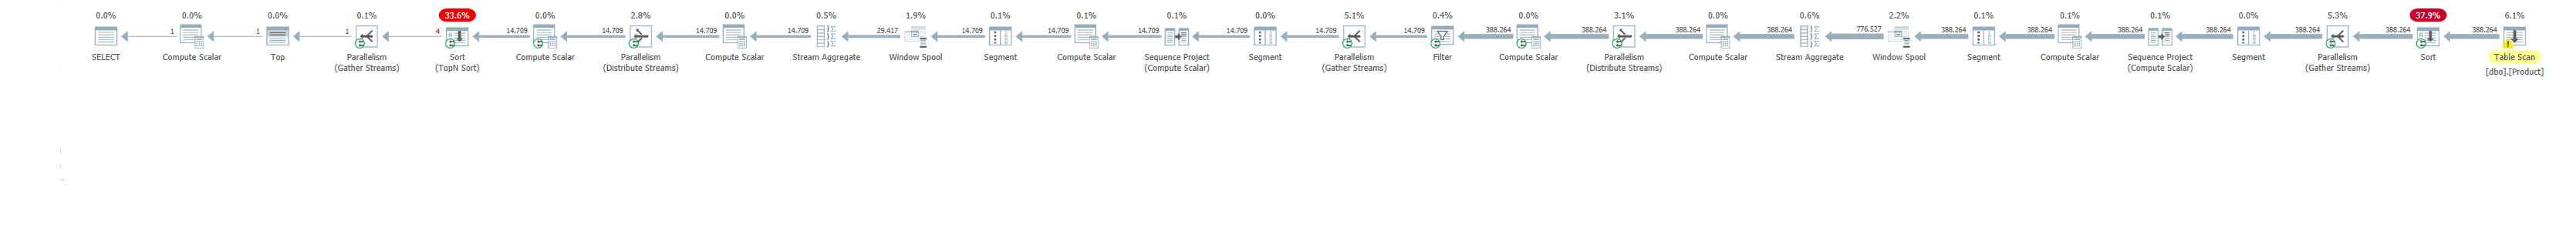
\includegraphics[width=1\textwidth]{image/joey/opdracht-05a.PNG}
    \caption{Queryplan Opdracht 05 Versie 02}
\end{figure}


\subsubsection{Versie 03}
In de eerste CTE worden de rijnummers, en de product\_id weergegven en in de 3e kolom word het verschil tussen deze 2 weergegeven.
Wanneer deze diff verschilt van de vorige diff waarde weet je dat er een gap is.
In de tweede CTE word er eerst gegroepeerd op de diff waarde. Nu hebben we alle islands gegroepeerd.
Vervolgens pakken we de hoogste en laagste waarde van een island, en berekenen we de lengte.
Als laatste stap halen we de hoogste waarde voor lengte er uit, en presenteren we die.

\lstinputlisting[language=SQL]{sql/nick/opdracht-01-05a.sql}
\begin{figure}
    \centering
    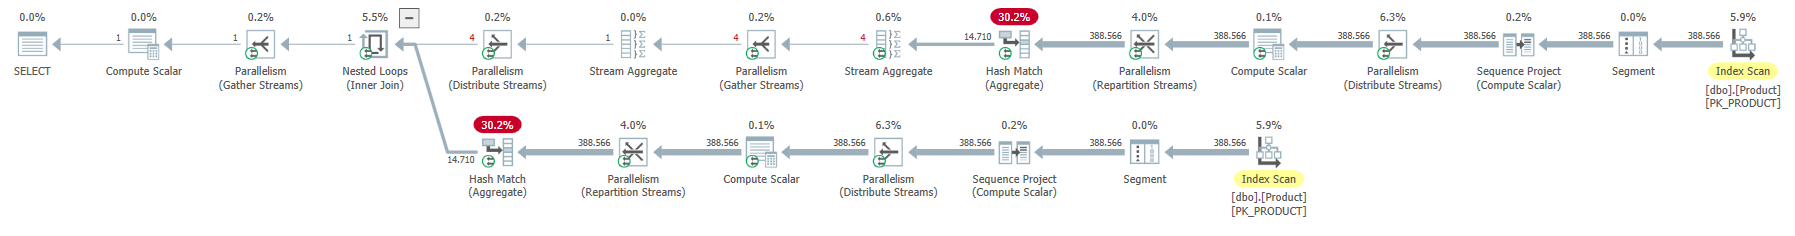
\includegraphics[width=1\textwidth]{image/nick/opdracht-05a.PNG}
    \caption{Queryplan Opdracht 05 Versie 02}
\end{figure}


\subsubsection{Conclusie}

\begin{tabular}{ || l | l | l | l | l | l | l | l | l | l | l | l | 1 | 1 | l | 1 | 1 || }
    \hline
    \textbf{Statement} & \textbf{Est Cost \%} & \textbf{Compile Time} & \textbf{Duration} & \textbf{CPU} & \textbf{Est CPU Cost \%} & \textbf{Est IO Cost \%} \\
    \hline
    \hline
    Versie03  & 36,5\%  & 19  & 3.154  & 5.022  & 36,2\% & 40,0\%  \\
    Versie02  & 27,0\%  & 9  & 2.357  & 2.973  & 25,5\% & 20,7\% \\
    Versie01  & 36,5\%  & 10  & 1.848  & 3.215  & 36,2\% & 39,4\%  \\
    \hline
    \hline
    \hline
\end{tabular}
\newline
\newline
\begin{tabular}{ || l | l | l | l | l | l | l | l | l | l | l | l | 1 | 1 | l | 1 | 1 || }
    \hline
    \textbf{Statement} &  \textbf{Est Rows} & \textbf{Actual Rows} & \textbf{RID Lookups} & \textbf{Parallel} & \textbf{Sort} & \textbf{Table Scan} & \textbf{Hash Match} \\
    \hline
    \hline
    Versie03  & 1        & 1  & 0  & 19  & 2  & 2  & 2 \\
    Versie02  & 1        & 1  & 0  & 10  & 2  & 1  & 0 \\
    Versie01  & 388.403  & 1  & 0  & 21  & 2  & 2  & 2 \\
    \hline
    \hline
    \hline
\end{tabular}


Doordat in de index de product\_type niet is meegenomen, zie je dat er Table Scans met een Sort word uitgevoerd op een grote tabel.
Dit brengt de nodige vertraging met zich mee, alleen ontkomen alle 3 versie's hier niet aan.
Maar toch is de performance van versie 02 een stukje beter.

De reden
    \clearpage
    \subsection{Opdracht 05a}
Geef ook het statement dat de langste reeks geeft die NIET in de database aanwezig is. Geef van beide statements het start en eind ID van de reeks.

\subsubsection{Versie 01}
In onderstaande query wordt er gebruik gemaakt van een CTE. Allereerst wordt de huidige ID vastgesteld. Vervolgens wordt er in deze
CTE gebruik gemaakt van een LAG functie, waardoor het verschil tussen de huidige ID en de vorige ID in de resultset kan worden vastgesteld.
Hierna wordt de grootte van dit verschil berekend door de vorige ID van de huidige ID af te trekken. Dit levert een waarde op welke
de maximale reeks met lege waarden bevat.
\lstinputlisting[language=SQL]{sql/marc/opdracht-01-05b.sql}
\begin{figure}
    \centering
    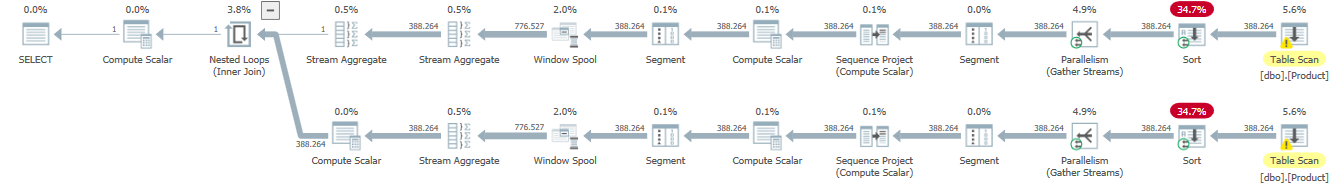
\includegraphics[width=1\textwidth]{image/marc/opdracht-05b.PNG}
    \caption{Queryplan Opdracht 05b Versie 02}
\end{figure}

\subsubsection{Versie 02}
TODO: Joey
\lstinputlisting[language=SQL]{sql/joey/opdracht-01-05b.sql}
\begin{figure}
    \centering
    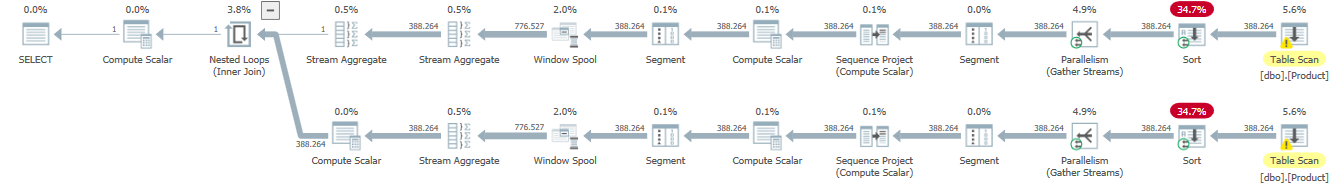
\includegraphics[width=1\textwidth]{image/marc/opdracht-05b.PNG}
    \caption{Queryplan Opdracht 05b Versie 02}
\end{figure}

\subsection{Conclusie}
Kijkende naar bovenstaande query plannen, kan worden gesteld dat versie 02 met 46\% net iets sneller is dan versie 01. In beide versies
is gebruik gemaakt van een CTE, in versie 01 wordt echter tweemaal gebruik gemaakt van de LAG functie om het verschil tussen de huidige
en de vorige rij in de resultset vast te stellen. Dit maakt deze query trager, wat ook blijkt uit het query plan. In het query plan van
versie 01 is te zien dat de LAG functie er tweemaal voor zorgt dat er een 'Tablescan' plaatsvind op de Product tabel. Deze gegevens worden
na deze 'Tablescan' allereerst gesorteerd middels een 'Sort'. Deze 'Sort' verbruikt beide keren 34,7\% van de query tijd, wat neer komt op
een totaal van 69,4\% van de gehele duur van de query. Ook versie 02 voert een 'Tablescan' op de Product tabel uit, echter wordt dit binnen
deze query maar één keer uitgevoerd. Hetzelfde geldt voor de hierop volgende 'Sort'.\\
\\
In versie 02 wordt er gebruik gemaakt van een TOP 1. Deze query is dus niet ANSI SQL. Bij versie 01 wordt op basis van de CTE het maximale
verschil vastgesteld.\\
\\
Gezien bovenstaande kan worden gesteld dat versie 01 in dit geval wellicht toch de beste optie is.
Wanneer beide queries in één batch worden uitgevoerd zijn de verschillen niet heel groot. Versie 01 is hierbij net wat trager, maar
voldoet wel aan de ANSI standaarden.\\
\\
\begin{tabular}{ || l | l | l | l | l | l | l | l | l | l | l | l | 1 | 1 | l | 1 | 1 || }
    \hline
    \textbf{Statement} & \textbf{Est Cost \%} & \textbf{Compile Time} & \textbf{Duration} &
    \textbf{CPU} & \textbf{Est CPU Cost \%} &
    \textbf{Est IO Cost \%} \\
    \hline
    \hline
    Versie01  & 54,0\%  & 12  & 1707  & 2370  & 52,6\% & 67,4\% \\
    \hline
    Versie02  & 46,0\%  & 8  & 958  & 1065  & 47,4\% & 67,4\%  \\
    \hline
\end{tabular}
\newline
\newline
\begin{tabular}{ || l | l | l | l | l | l | l | l | l | l | l | l | 1 | 1 | l | 1 | 1 || }
    \hline
    \textbf{Statement} &  \textbf{Est Rows} & \textbf{Actual Rows} & \textbf{RID Lookups} &
    \textbf{Parallel} & \textbf{Sort} &
    \textbf{Table Scan} & \textbf{Hash Match} \\
    \hline
    \hline
    Versie01  & 1  & 1  & 0  & 6  & 2  & 2  & 0 \\
    \hline
    Versie02  & 1  & 1  & 0  & 7  & 2  & 1  & 0 \\
    \hline
\end{tabular}
    \clearpage


    \section{Opdracht 2: Constraints}
    \paragraph{
    Implementeer onderstaande constraints.
    Het kan zijn dat je een aantal al tijdens de casus DDDQ heb ge�dentificeerd en/of zelfs al gemaakt.
    Lever in dat geval die code weer in voor deze casus. Indien je de constraints procedureel oplost, maak je zowel een Stored Procedure als een After Trigger.
    Zorg voor nette error handling in jouw code en schrijf een complete testset voor beide constraint implementaties.
    Leg uit of de SP of Trigger jouw voorkeur heeft en uiteraard waarom.
    Als je bij een constraint vindt dat een Instead Of Trigger de betere variant is, maak je die ook en leg je uit waarom dit de beste oplossing is voor deze constraint.

    }
    \label{opdracht2}
    \subsection{Opdracht 01}

Geef van een film, de hele reeks waar die bij hoort met volgnummer en in de juiste volgorde.
Indien hij niet in een reeks zit, is de lijst gewoon ��n lang met volgnummer 1.
Dit moet ��n statement worden die van een variabel ID de reeks geeft zoals onderstaand voorbeeld:
DECLARE @MovieInReeks INT = 207989;


\begin{lstlisting}
-- jouw statement hier levert onderstaand resultaat:

ITEM_ID		TITLE				Volgnummer
207992		Matrix, The				1
207989		Matrix Reloaded, The			2
207991		Matrix Revolutions, The		3
\end{lstlisting}

\subsubsection{Versie 01}

TODO: Marc

\lstinputlisting[language=SQL]{sql/marc/opdracht-01-01.sql}
\begin{figure}
    \centering
    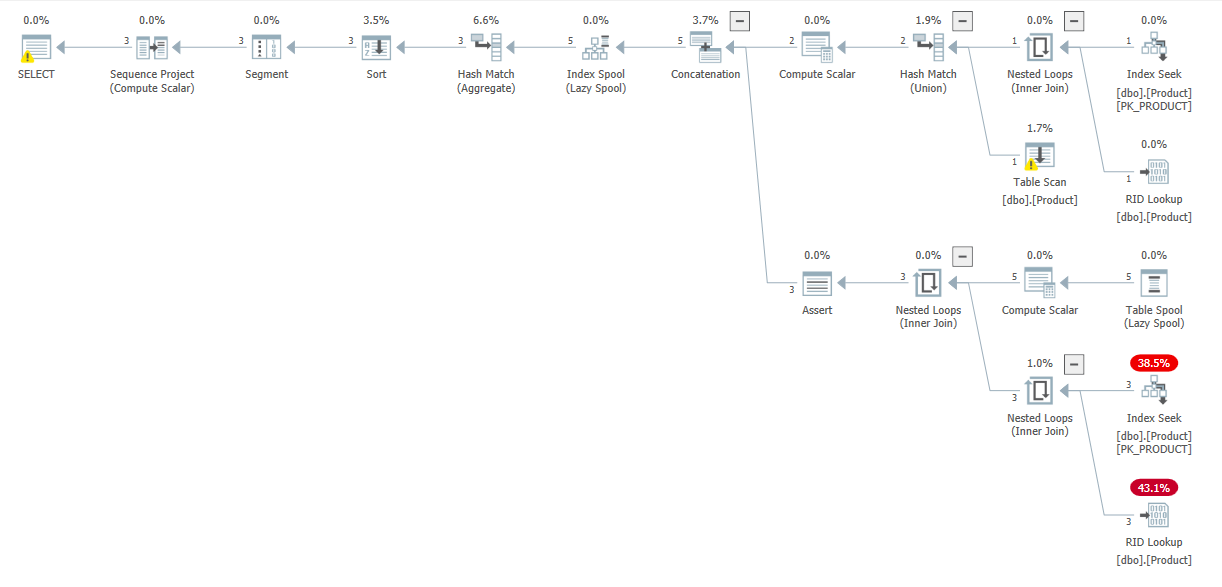
\includegraphics[width=1\textwidth]{image/marc/opdracht-01.PNG}
    \caption{Queryplan Opdracht 01 Versie 01}
\end{figure}

\subsubsection{Versie 02}
TODO: Joey

\lstinputlisting[language=SQL]{sql/joey/opdracht-01-01.sql}
\begin{figure}
    \centering
    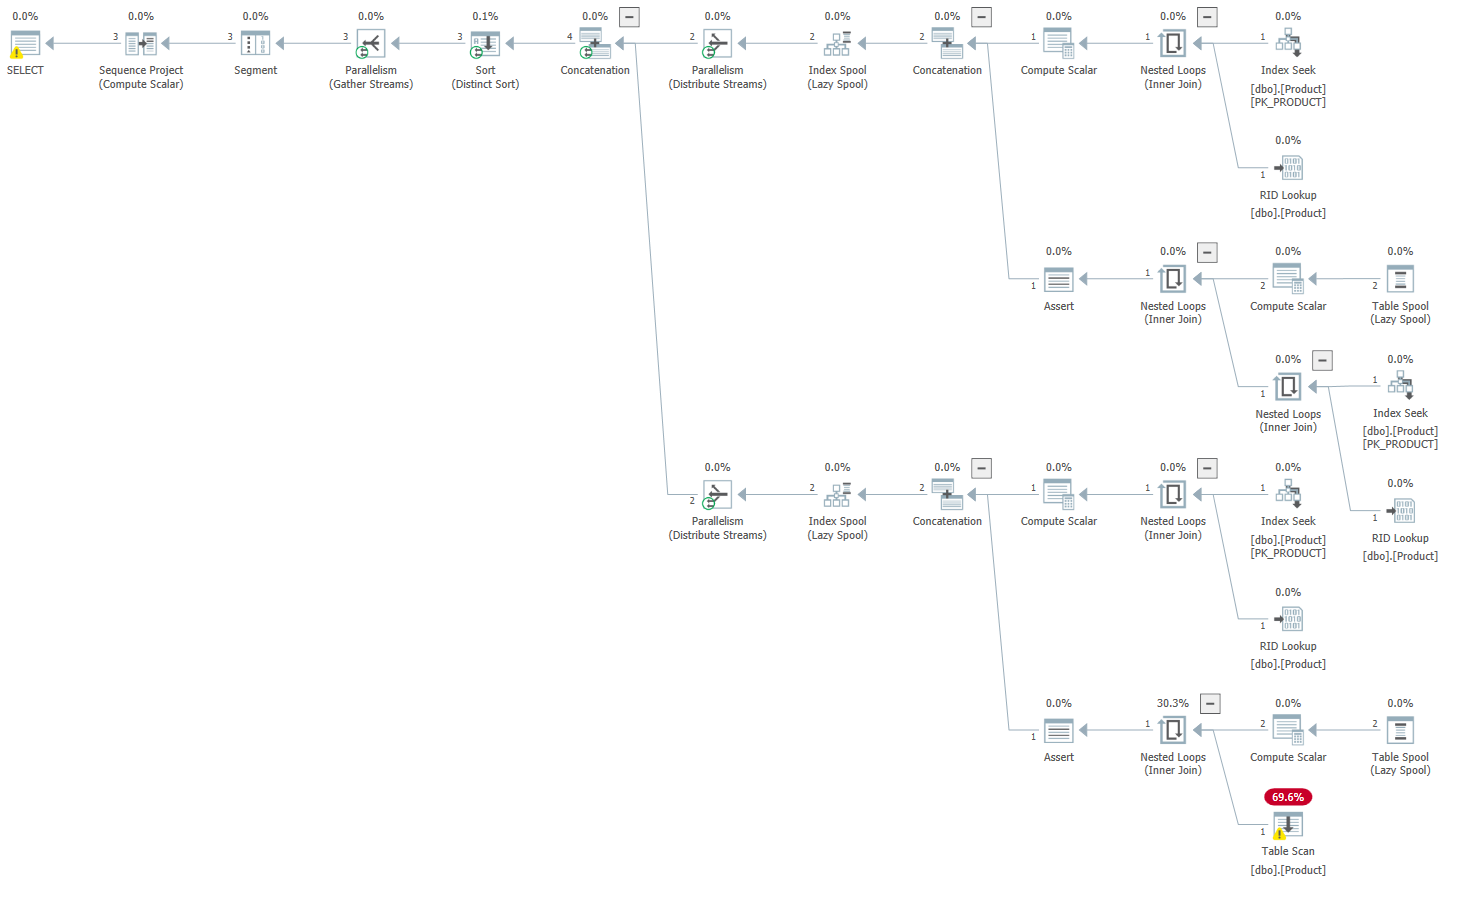
\includegraphics[width=1\textwidth]{image/joey/opdracht-01.PNG}
    \caption{Queryplan Opdracht 01 Versie 02}
\end{figure}


\subsubsection{Versie 03}

    De intentie van deze query was om geen CTE te gebruiken. In dit alternatief maken we gebruik van een tijdelijke tabel.
    Na het aanmaken van van de tijdelijke tabel worden er 2 while loops gedraaid. Bij de eerste loop word er gekeken of er een vorige film is.
    Als die er is, word die opgeslagen in de tijdelijke tabel, en herhaald hij de loop tot het punt komt dat er geen vorige film meer is.
    Hetzelfde doet hij met vervolg films, als deze er zijn word die ook in de tijdelijke tabel opgeslagen.
    Uiteindelijk word de tijdelijke tabel uitgevraagd, en krijg je de lijst met films te zien.
    Als laatste word de tijdelijke tabel verwijderd.

\lstinputlisting[language=SQL]{sql/nick/opdracht-01-01.sql}

\subsubsection{Conclusie}

\begin{tabular}{ || l | l | l | l | l | l | l | l | l | l | l | l | 1 | 1 | l | 1 | 1 || }
    \hline
    \textbf{Statement} & \textbf{Est Cost \%} & \textbf{Compile Time} & \textbf{Duration} &
    \textbf{CPU} & \textbf{Est CPU Cost \%} &
    \textbf{Est IO Cost \%} \\
    \hline
    \hline
    Versie01  & 0,0\%  & 12  & 40  & 40  & 4,9\% & 0,0\% \\
    \hline
    Versie02  & 100,0\%  & 20  & 76  & 75  & 95,1\% & 100,0\%  \\
    \hline
\end{tabular}
\newline
\newline
\begin{tabular}{ || l | l | l | l | l | l | l | l | l | l | l | l | 1 | 1 | l | 1 | 1 || }
    \hline
    \textbf{Statement} &  \textbf{Est Rows} & \textbf{Actual Rows} & \textbf{RID Lookups} &
    \textbf{Parallel} & \textbf{Sort} &
    \textbf{Table Scan} & \textbf{Hash Match} \\
    \hline
    \hline
    Versie01  & 77.765  & 3  & 2  & 0  & 1  & 1  & 2 \\
    \hline
    Versie02  & 1.157.780  & 3  & 3  & 5  & 1  & 1  & 0 \\
    \hline
\end{tabular}


HIer komt dus een lang verhaal over welke query het beste is, en waarom

    \clearpage

    \section{Opdracht 3: Transactie management en Concurrency}
    \paragraph{
        In zowel jouw SP's als Triggers maak je correct gebruik van Transacties.
        Kies het juiste isolation level bij een implementatie en leg uit waarom dat het juiste level is.
        Leg hierbij uit welke problemen zich kunnen voordoen in het default isolation level, hoe locking in die situatie werkt en hoe die d.m.v. het isolation level aangepast wordt.
    }
    \label{opdracht3}
    \subsection{Opdracht 01}

Geef van een film, de hele reeks waar die bij hoort met volgnummer en in de juiste volgorde.
Indien hij niet in een reeks zit, is de lijst gewoon ��n lang met volgnummer 1.
Dit moet ��n statement worden die van een variabel ID de reeks geeft zoals onderstaand voorbeeld:
DECLARE @MovieInReeks INT = 207989;


\begin{lstlisting}
-- jouw statement hier levert onderstaand resultaat:

ITEM_ID		TITLE				Volgnummer
207992		Matrix, The				1
207989		Matrix Reloaded, The			2
207991		Matrix Revolutions, The		3
\end{lstlisting}

\subsubsection{Versie 01}

TODO: Marc

\lstinputlisting[language=SQL]{sql/marc/opdracht-01-01.sql}
\begin{figure}
    \centering
    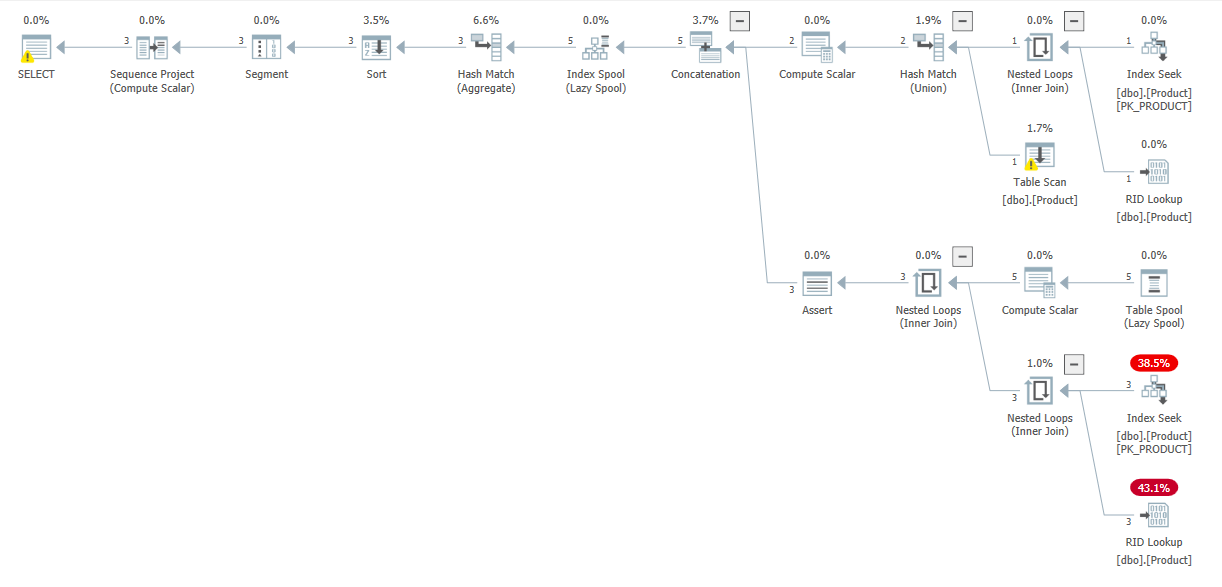
\includegraphics[width=1\textwidth]{image/marc/opdracht-01.PNG}
    \caption{Queryplan Opdracht 01 Versie 01}
\end{figure}

\subsubsection{Versie 02}
TODO: Joey

\lstinputlisting[language=SQL]{sql/joey/opdracht-01-01.sql}
\begin{figure}
    \centering
    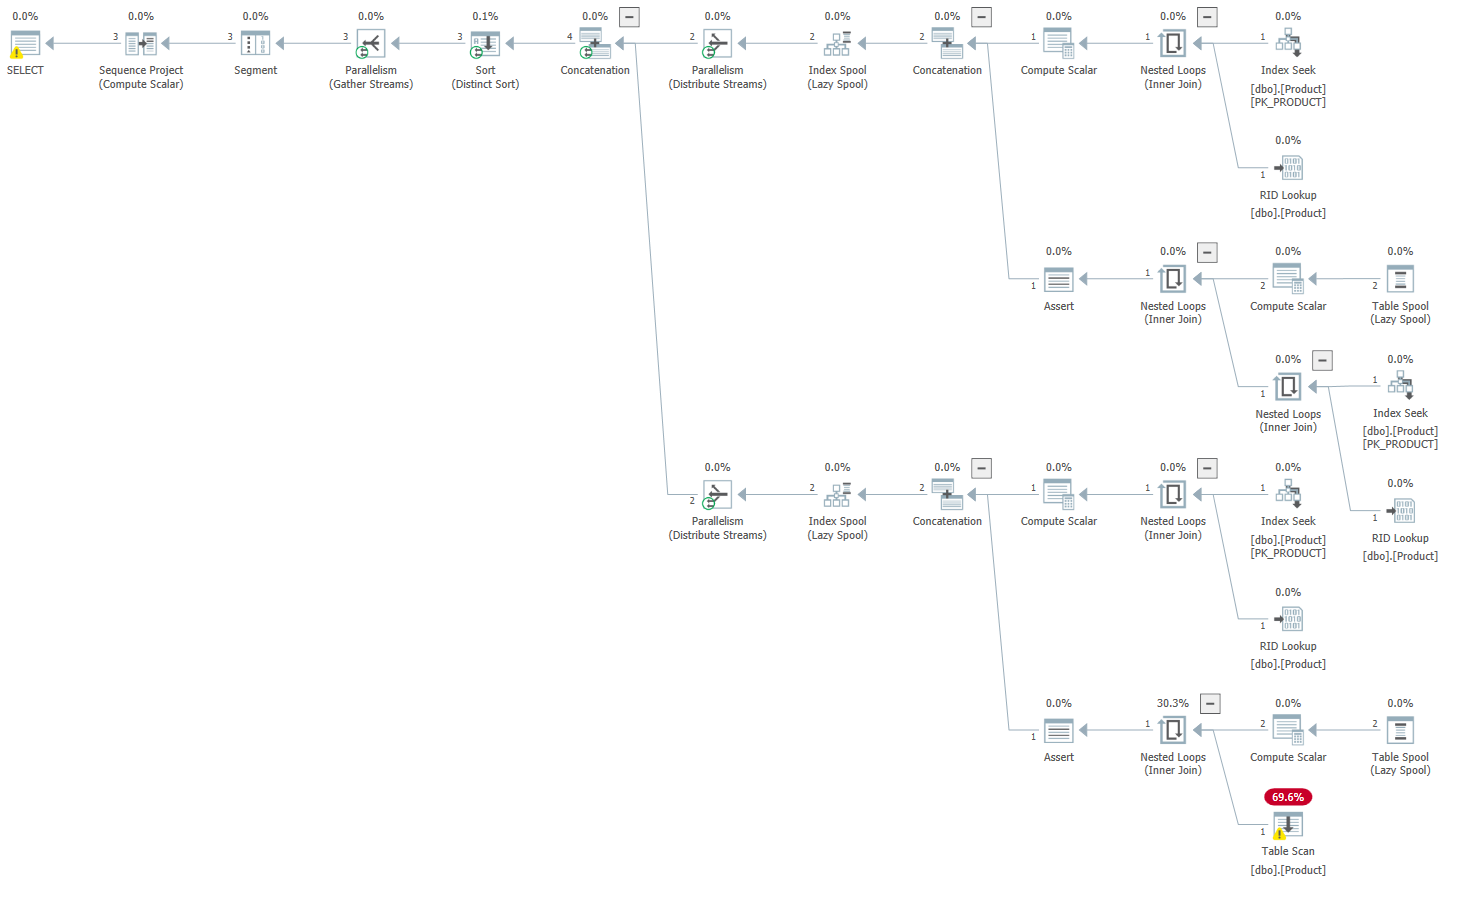
\includegraphics[width=1\textwidth]{image/joey/opdracht-01.PNG}
    \caption{Queryplan Opdracht 01 Versie 02}
\end{figure}


\subsubsection{Versie 03}

    De intentie van deze query was om geen CTE te gebruiken. In dit alternatief maken we gebruik van een tijdelijke tabel.
    Na het aanmaken van van de tijdelijke tabel worden er 2 while loops gedraaid. Bij de eerste loop word er gekeken of er een vorige film is.
    Als die er is, word die opgeslagen in de tijdelijke tabel, en herhaald hij de loop tot het punt komt dat er geen vorige film meer is.
    Hetzelfde doet hij met vervolg films, als deze er zijn word die ook in de tijdelijke tabel opgeslagen.
    Uiteindelijk word de tijdelijke tabel uitgevraagd, en krijg je de lijst met films te zien.
    Als laatste word de tijdelijke tabel verwijderd.

\lstinputlisting[language=SQL]{sql/nick/opdracht-01-01.sql}

\subsubsection{Conclusie}

\begin{tabular}{ || l | l | l | l | l | l | l | l | l | l | l | l | 1 | 1 | l | 1 | 1 || }
    \hline
    \textbf{Statement} & \textbf{Est Cost \%} & \textbf{Compile Time} & \textbf{Duration} &
    \textbf{CPU} & \textbf{Est CPU Cost \%} &
    \textbf{Est IO Cost \%} \\
    \hline
    \hline
    Versie01  & 0,0\%  & 12  & 40  & 40  & 4,9\% & 0,0\% \\
    \hline
    Versie02  & 100,0\%  & 20  & 76  & 75  & 95,1\% & 100,0\%  \\
    \hline
\end{tabular}
\newline
\newline
\begin{tabular}{ || l | l | l | l | l | l | l | l | l | l | l | l | 1 | 1 | l | 1 | 1 || }
    \hline
    \textbf{Statement} &  \textbf{Est Rows} & \textbf{Actual Rows} & \textbf{RID Lookups} &
    \textbf{Parallel} & \textbf{Sort} &
    \textbf{Table Scan} & \textbf{Hash Match} \\
    \hline
    \hline
    Versie01  & 77.765  & 3  & 2  & 0  & 1  & 1  & 2 \\
    \hline
    Versie02  & 1.157.780  & 3  & 3  & 5  & 1  & 1  & 0 \\
    \hline
\end{tabular}


HIer komt dus een lang verhaal over welke query het beste is, en waarom

    \clearpage

    \section{Opdracht 4: Indexeren}
    \paragraph{
        Geef aan waar jij denkt dat indexen nuttig kunnen zijn.
        Toon het verschil aan tussen de situatie met en zonder index en verklaar de verschillen in performance en queryplannen.
        Mogelijk veranderd je keuze van query als je gebruik maakt van indexen, geef dat dan aan.
    }
    \label{opdracht4}
    \subsection{Opdracht 01}

Geef van een film, de hele reeks waar die bij hoort met volgnummer en in de juiste volgorde.
Indien hij niet in een reeks zit, is de lijst gewoon ��n lang met volgnummer 1.
Dit moet ��n statement worden die van een variabel ID de reeks geeft zoals onderstaand voorbeeld:
DECLARE @MovieInReeks INT = 207989;


\begin{lstlisting}
-- jouw statement hier levert onderstaand resultaat:

ITEM_ID		TITLE				Volgnummer
207992		Matrix, The				1
207989		Matrix Reloaded, The			2
207991		Matrix Revolutions, The		3
\end{lstlisting}

\subsubsection{Versie 01}

TODO: Marc

\lstinputlisting[language=SQL]{sql/marc/opdracht-01-01.sql}
\begin{figure}
    \centering
    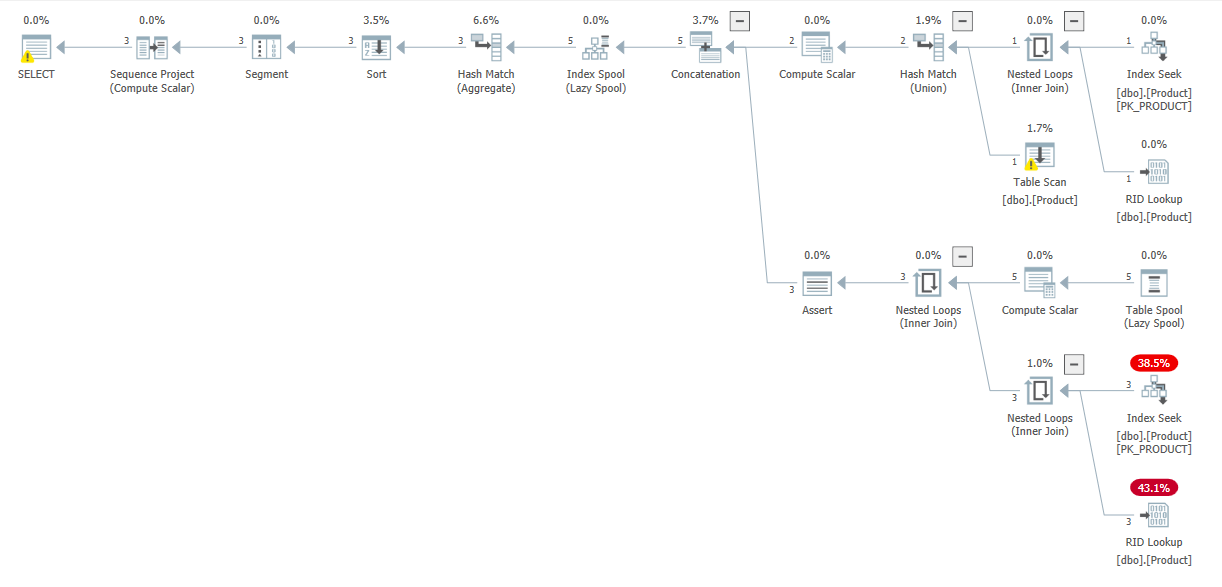
\includegraphics[width=1\textwidth]{image/marc/opdracht-01.PNG}
    \caption{Queryplan Opdracht 01 Versie 01}
\end{figure}

\subsubsection{Versie 02}
TODO: Joey

\lstinputlisting[language=SQL]{sql/joey/opdracht-01-01.sql}
\begin{figure}
    \centering
    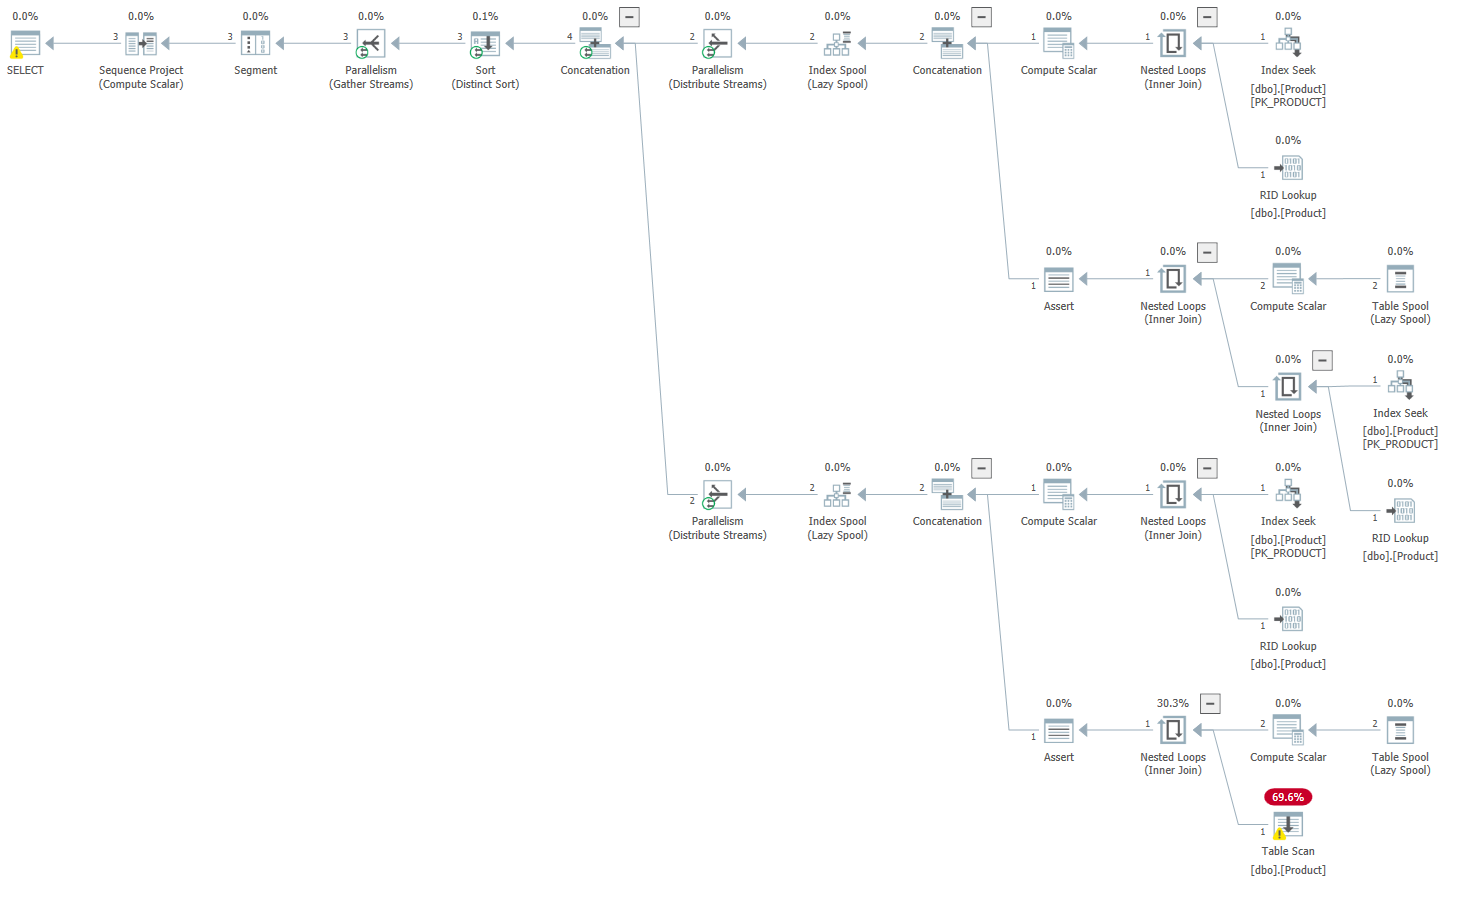
\includegraphics[width=1\textwidth]{image/joey/opdracht-01.PNG}
    \caption{Queryplan Opdracht 01 Versie 02}
\end{figure}


\subsubsection{Versie 03}

    De intentie van deze query was om geen CTE te gebruiken. In dit alternatief maken we gebruik van een tijdelijke tabel.
    Na het aanmaken van van de tijdelijke tabel worden er 2 while loops gedraaid. Bij de eerste loop word er gekeken of er een vorige film is.
    Als die er is, word die opgeslagen in de tijdelijke tabel, en herhaald hij de loop tot het punt komt dat er geen vorige film meer is.
    Hetzelfde doet hij met vervolg films, als deze er zijn word die ook in de tijdelijke tabel opgeslagen.
    Uiteindelijk word de tijdelijke tabel uitgevraagd, en krijg je de lijst met films te zien.
    Als laatste word de tijdelijke tabel verwijderd.

\lstinputlisting[language=SQL]{sql/nick/opdracht-01-01.sql}

\subsubsection{Conclusie}

\begin{tabular}{ || l | l | l | l | l | l | l | l | l | l | l | l | 1 | 1 | l | 1 | 1 || }
    \hline
    \textbf{Statement} & \textbf{Est Cost \%} & \textbf{Compile Time} & \textbf{Duration} &
    \textbf{CPU} & \textbf{Est CPU Cost \%} &
    \textbf{Est IO Cost \%} \\
    \hline
    \hline
    Versie01  & 0,0\%  & 12  & 40  & 40  & 4,9\% & 0,0\% \\
    \hline
    Versie02  & 100,0\%  & 20  & 76  & 75  & 95,1\% & 100,0\%  \\
    \hline
\end{tabular}
\newline
\newline
\begin{tabular}{ || l | l | l | l | l | l | l | l | l | l | l | l | 1 | 1 | l | 1 | 1 || }
    \hline
    \textbf{Statement} &  \textbf{Est Rows} & \textbf{Actual Rows} & \textbf{RID Lookups} &
    \textbf{Parallel} & \textbf{Sort} &
    \textbf{Table Scan} & \textbf{Hash Match} \\
    \hline
    \hline
    Versie01  & 77.765  & 3  & 2  & 0  & 1  & 1  & 2 \\
    \hline
    Versie02  & 1.157.780  & 3  & 3  & 5  & 1  & 1  & 0 \\
    \hline
\end{tabular}


HIer komt dus een lang verhaal over welke query het beste is, en waarom

    \clearpage

    %=================o ~~
    \newpage
    \section{Bronvermelding}
    \label{bronvermelding}

    \nocite{*}

\end{document}